\documentclass{jsarticle}
\usepackage[dvipdfmx]{graphicx}
\begin{document}
In recent years, alongside experimental approaches, simulations utilizing computational tools have been employed to investigate intracellular signaling processes. Simulation research, which seeks to validate hypotheses based on experimental results, is increasingly recognized as a valuable complement to experimental studies. In this paper, we reevaluate the hypothesis that regulatory T cells are involved in the transition from inflammatory microglia to anti-inflammatory microglia from a mathematical modeling (kinetics) standpoint. 
We denote the quantities of inflammatory microglia, anti-inflammatory microglia, and regulatory T cells as M1, M2, and Treg, respectively. Here, we describe the dynamics of M1, M2, and Treg using the following rate equations as the simplest scenario:
\begin{eqnarray}
  \label{eqn:01}
  \frac{dM_{1}(t)}{dt} &=& \alpha f_1(t)- \beta f_2(M_1, T_{reg}) \\
  \label{eqn:02}
  \frac{dM_2(t)}{dt} &=& \beta f_2(M_1, T_{reg}) \\
  \label{eqn:03}
  \frac{dT_{reg}}{dt} &=& f_3(t).
\end{eqnarray}
(\ref{eqn:01})式は$M_1$の動態を表す.敗血症時にマイクログリアがある上限まで単調増加するという観察結果から$f_1(t)$は上限のある単調増加関数である.また,(\ref{eqn:01})の第2項は炎症性マイクログリアから,抗炎症性マイクログリアへの変化を意味し,$M_1$および$T_{reg}$に関する増加関数となる.(\ref{eqn:02})式は$M_2$の動態を表す.ここで,(\ref{eqn:01})$+$(\ref{eqn:02})は保存されることに注意する.最後に,(\ref{eqn:03})式は$T_{reg}$の動態を表す.敗血症時に制御性T細胞は増加し続けることが知られているため,$f_3>0$となる.図より,敗血症発生当初は炎症性マイクログリア($M_1$)が急峻に増加し,十分に$M_1$が大きくなったところで遅れて抗炎症性マイクログリア($M_2$)増加し,炎症性マイクログリア細胞が減少することになる.炎症性マイクログリアの減少率は$f_2$の形およびパラメータ$\beta$に強く依存する.これらを決定するためには制御性T細胞と抗炎症性マイクログリア機序を明らかにする必要がある.また,制御性T細胞と抗炎症性マイクログリア量の時系列を比較することで,定量的な予測が可能となる.

\begin{figure}[h]
  \centering
    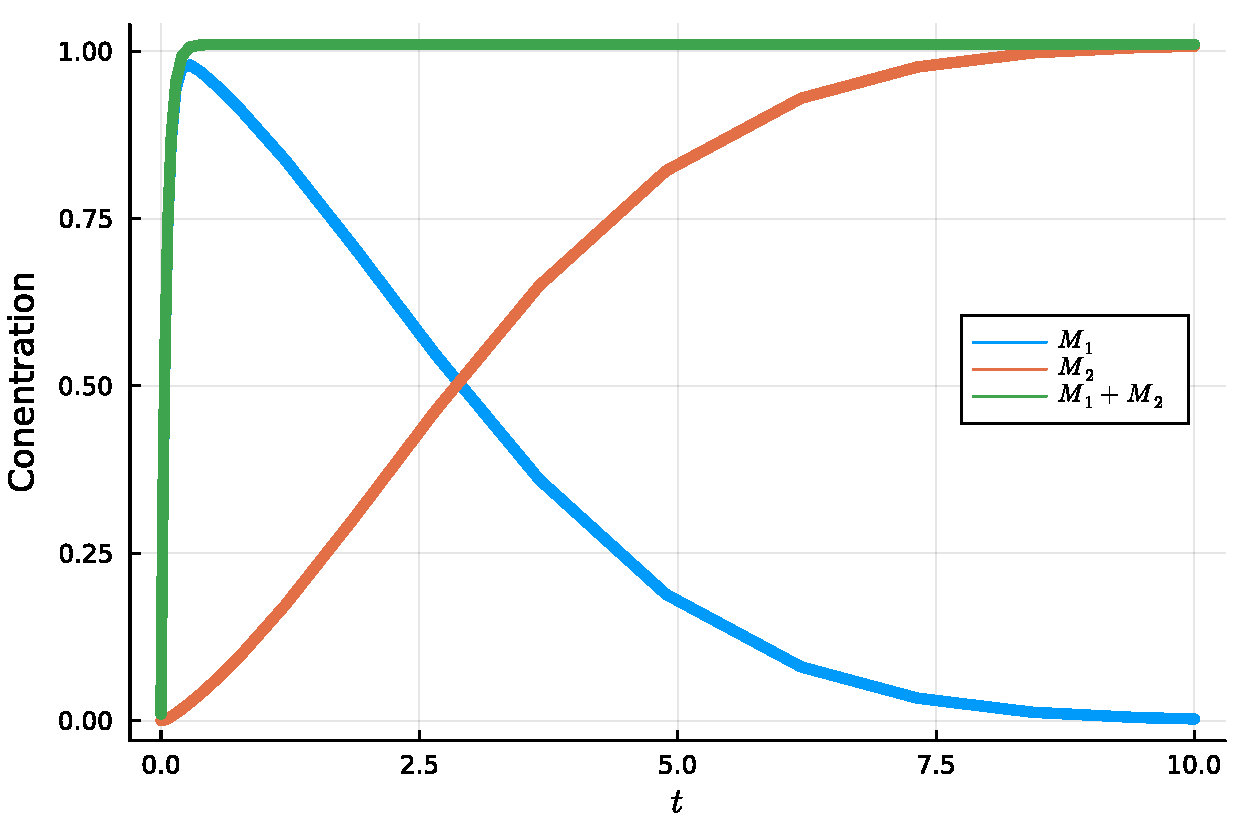
\includegraphics[width=12cm,clip]{../fig/masafig01.pdf}
        \caption{$M_1$, $M_2$, $M_1+M_2$の時系列.$\alpha=1.0$, $\beta=0.1$とし,関数形は$f_1(t):= \gamma\exp{(-\gamma T)}$,$f_2(M_1, T_{reg}):=M_1T_{reg}$とした,}
      \label{fig:01}
  \end{figure}

\end{document}